The first test is devoted to investigating the distribution of the velocities of the particles after sufficiently long time. From statistical mechanics, we know that the velocities of a $2$-dimensional gas at equilibrium will distribute according to Maxwell-Boltzmann's velocity distribution: 
\begin{equation}\label{eq:maxwell}
	p(v) = \frac{mv}{k_B T} \exp{\left(- \frac{mv^2}{2 k_B T}\right)},
\end{equation}
where $k_B$ is Boltzmann's constant, $T$ the absolute temperature, and $m$ the mass of the particles. It is evident that the particles will have to have the same mass for comparing with the known distribution in equation \ref{eq:maxwell}. The case of dissimilar masses is considered in section \ref{sec:mix1} and \ref{sec:mix2}.

We initialise an system of particles with velocities $\mathbf{v} = [v_0 \cos{\theta} , v_0 \sin{\theta}]$ with $\theta \sim \U[0,2\pi]$. The initial distribution of the velocities is therefore $\delta (v - v_0)$. After simulating the system until equilibrium is reached, i.e. the the average number of particle collision is $\gg 1$, the distribution is as shown in figure \ref{fig:dist_1}. For this simulation, the stop criterion used was that the average number of collisions surpassed $50$. To get a larger number of independent samples, I have used the speeds at $20$ different times in this simulation sampled such that all particles have collided a few times between each sample. 

\begin{figure}[htb]
	\centering
	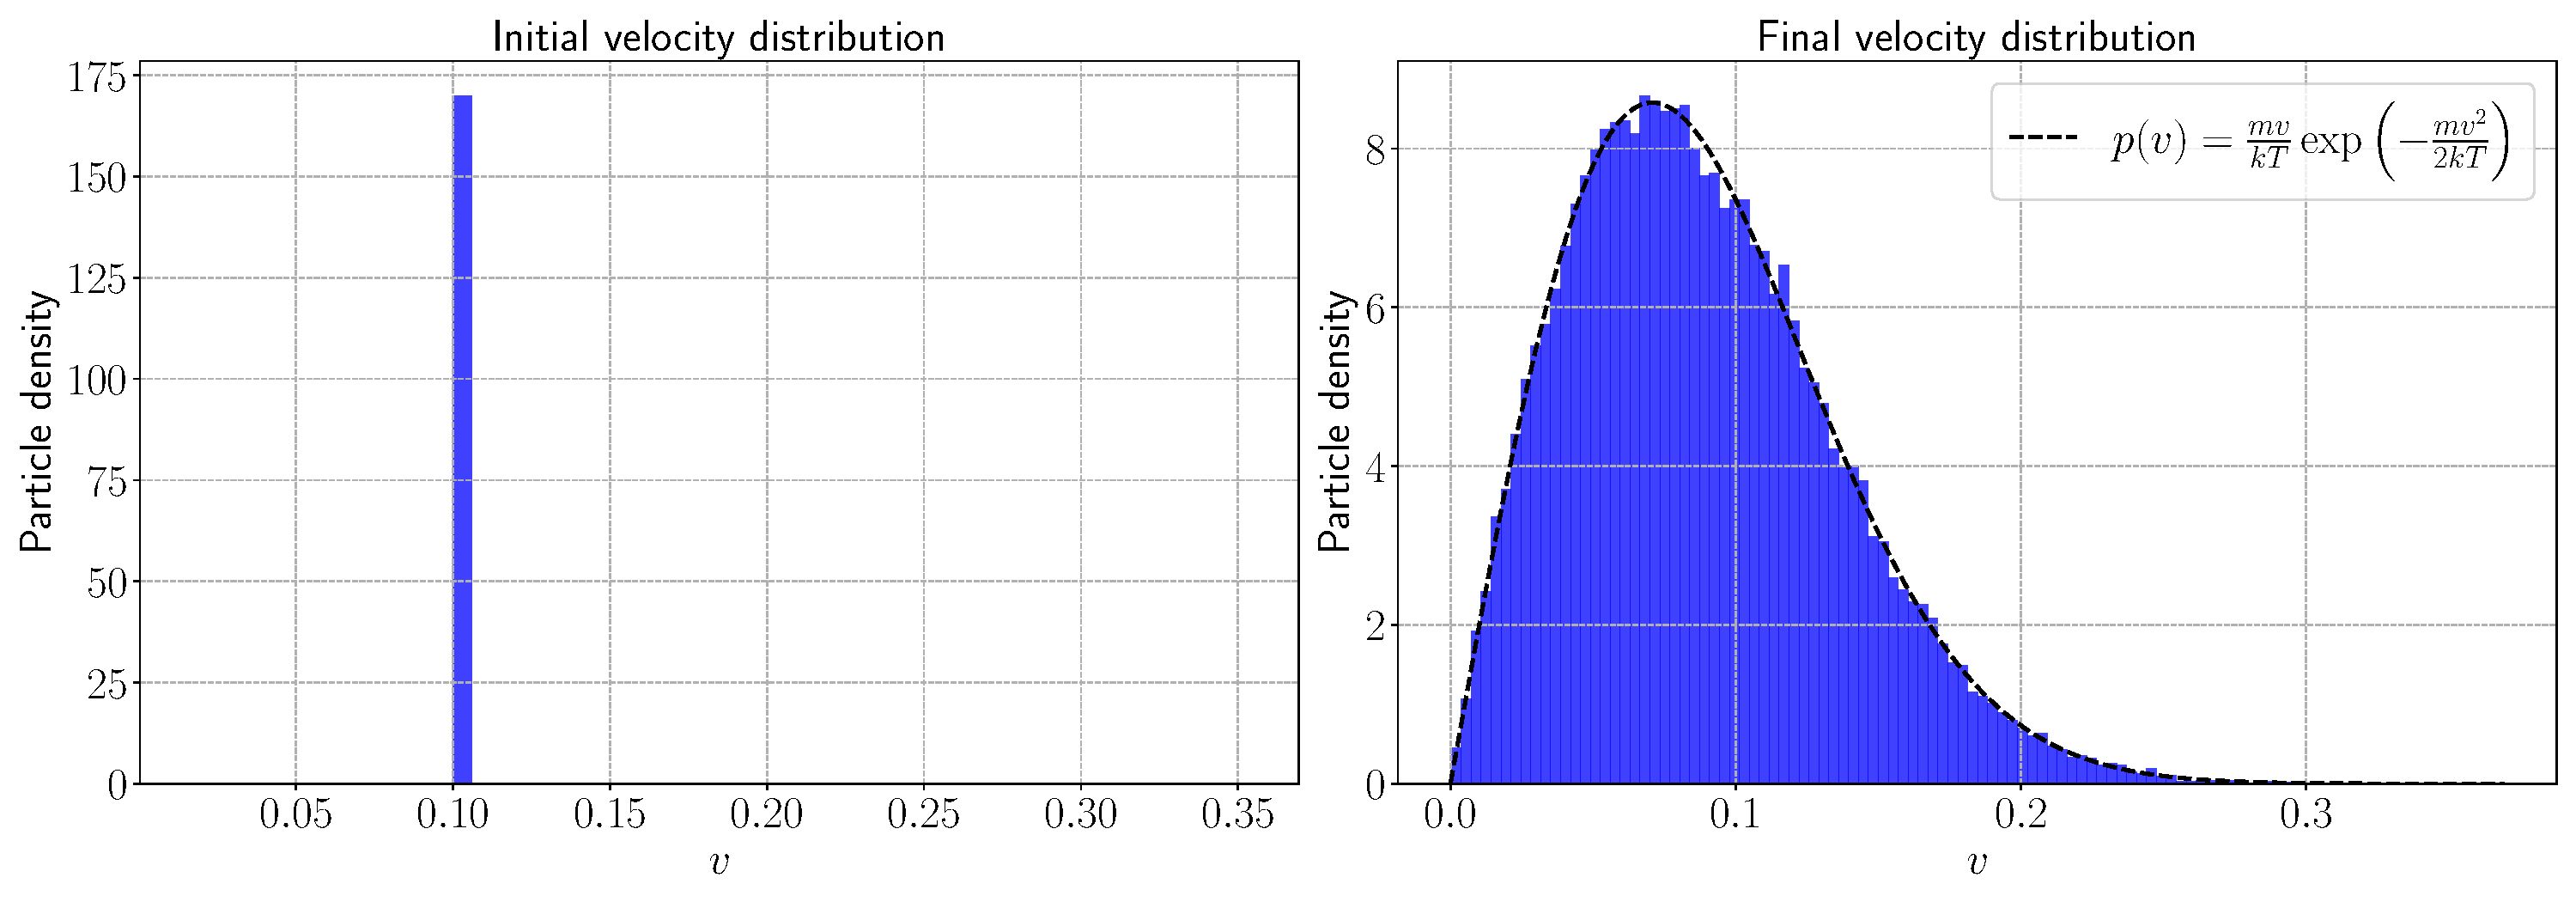
\includegraphics[width=\textwidth]{../fig/distribution}
	\caption{Distribution of velocities in a gas of $50000$ particles.}
	\label{fig:dist_1}
\end{figure}

%To make the comparison more quantitative, we plot the difference between the Gaussian kernel density estimation of the final distribution and the Maxwell distribution. This is shown in figure \ref{fig:dist_2}. 
%
%\begin{figure}[htb]
%	\centering
%	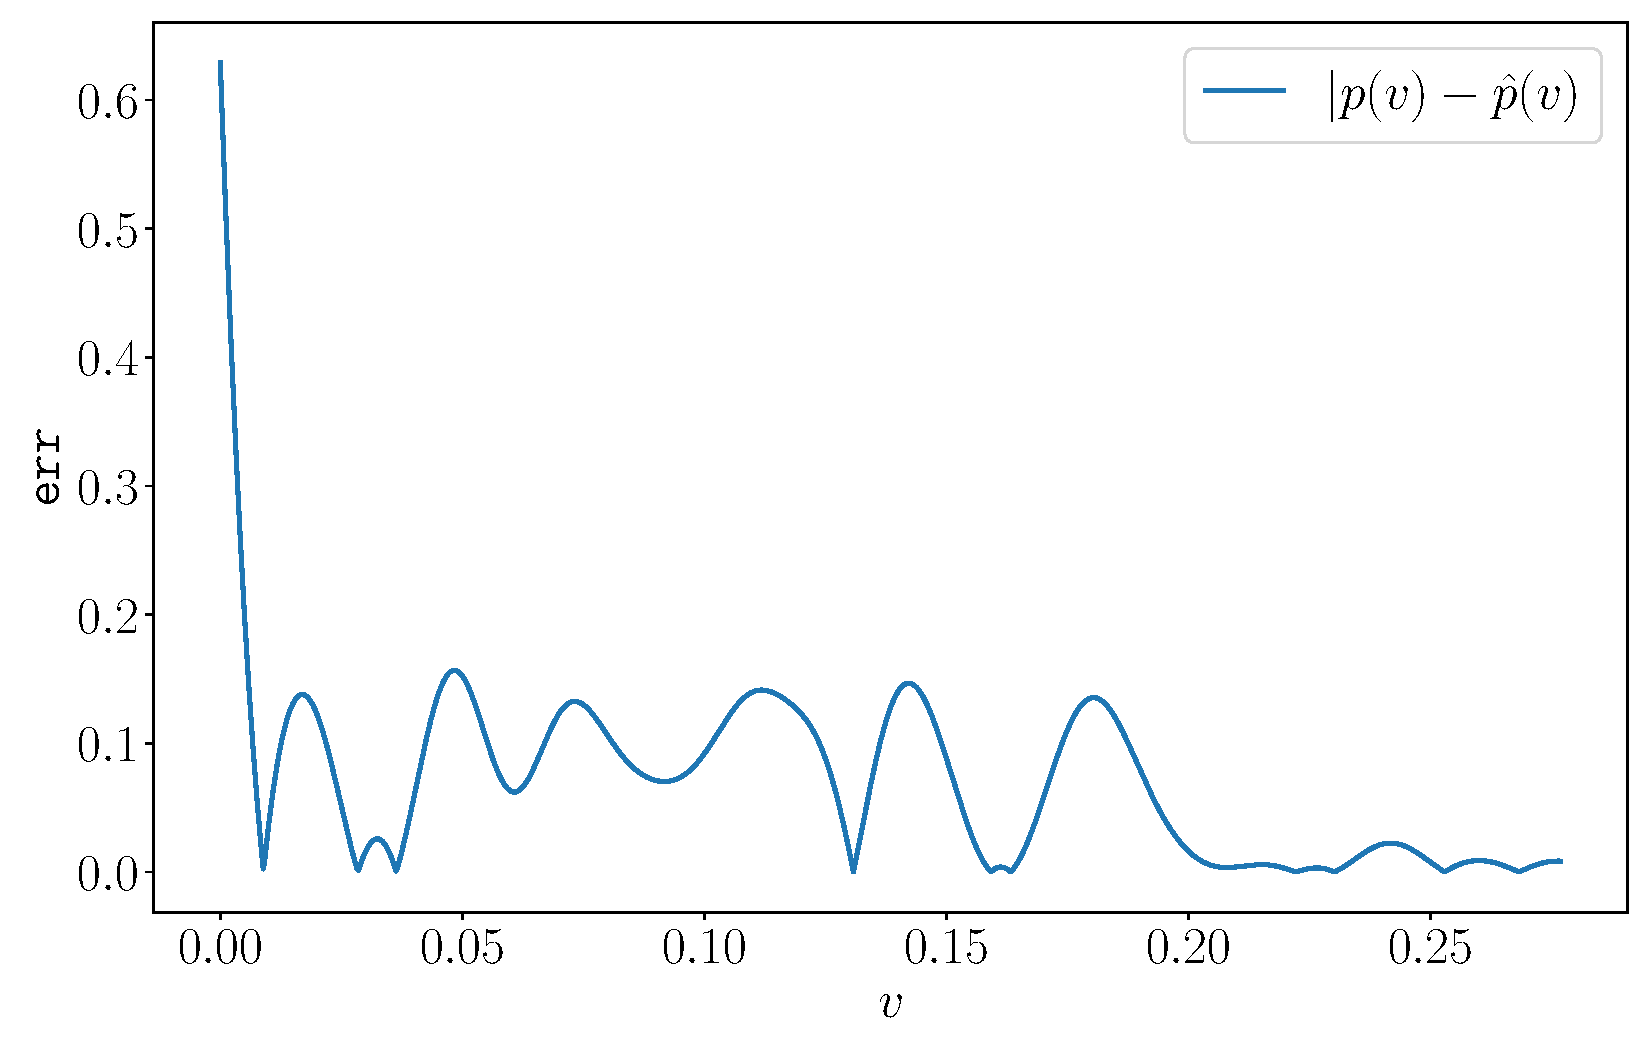
\includegraphics[width=0.8\textwidth]{../fig/kde_diff}
%	\caption{Deviation between Gaussian kernel density estimation of the velocity distribution, $\hat{p}(v)$ and the Maxwell-distribution $p(v)$.}
%	\label{fig:dist_2}
%\end{figure}

To have a more quantitative measure of how good the fit is, divide the real line into $k$ intervals and consider the normalized $\ell^1$-norm of the difference at each interval 
\begin{equation}\label{eq:err}
	\texttt{err} = \frac{1}{2} \sum_{j=1}^{k} \rvert d_j - p_j\lvert,
\end{equation}
where $d_j$ denotes the density of samples in interval $I_j$ and 
\[
	p_j = \int_{I_j} p(v) \, \text{d}v
\]
is the probability that an observation falls into interval $I_j$. It is evident from equation \ref{eq:err} that $\texttt{err}\in [0,1]$. For the distribution shown in figure \ref{fig:dist_1} $\texttt{err} \approx  0.0078527$. This indicates a good fit with the known distribution.

%This test is constructed as follows:
%
%Divide the real line line into $k$ disjoint intervals $I_1, \dots, I_k$. For $j = 1, \dots, k$, let 
%	\[
%		p_j(\boldsymbol{\theta}) = \int_{I_j} p(v;\boldsymbol{\theta}) \, \text{d}v
%	\]
%be the probability that an observation falls into interval $I_j$ of the model. Here $\boldsymbol{\theta} = (\theta_1, \dots, \theta_s)$ denotes the parameters of the model. Let $N_j$ be the number of test samples out of $n$ that fall into interval $I_j$. Define the following test-statistic
%
%\begin{equation}\label{eq:Q}
%	Q := \sum_{j=1}^{k} \frac{\left( N_j - np_j(\boldsymbol{\theta}) \right)^2}{n p_j(\boldsymbol{\theta})}.
%\end{equation}
%
%The following theorem provides a test we can do on the data.
%
%\begin{thm}
%	The test statistic $Q$ in equation \ref{eq:Q} converges to a $\chi^2_{k-1-s}$ random variable.
%\end{thm}
%
%Hence, by calculating the observed value of $Q$, $q$, an approximate $p$-value for the test that the data are \texttt{IID} and drawn from the assumed model is $\mathbb{P}(\chi^2_{k-1-s} > q)$. Performing this for the distribution shown in figure \ref{fig:dist_1} yields a $p$-value of $0$. Note that this only gives us a good reason \textit{not} to conclude that the data is \textit{not} drawn from the assumed model. 